\subsection{Estación de baja densidad}

%En entornos urbanos donde las estaciones ferroviarias se encuentran separadas entre sí por unos pocos kilómetros es necesaria una interconectividad mayor. El sistema ferroviario debe satisfacer la demanda de una población mayor y a la vez coexistir con un trazado vehicular mucho mas denso que cruza al trazado ferroviario en varios puntos. En este contexto, una topología simple como la presentada en la Figura \ref{fig:simple_1} es una solución óptima al problema planteado.

En entornos urbanos donde las estaciones ferroviarias se encuentran separadas entre sí por unos pocos kilómetros es necesaria una interconectividad mayor. Si por la estación ferroviaria solamente pasan uno o dos ramales ferroviarias, una topología de estación de baja densidad como la ilustrada en la Figura \ref{fig:simple_1} es una solución óptima al problema planteado.

    \begin{figure}[H]
        \centering
        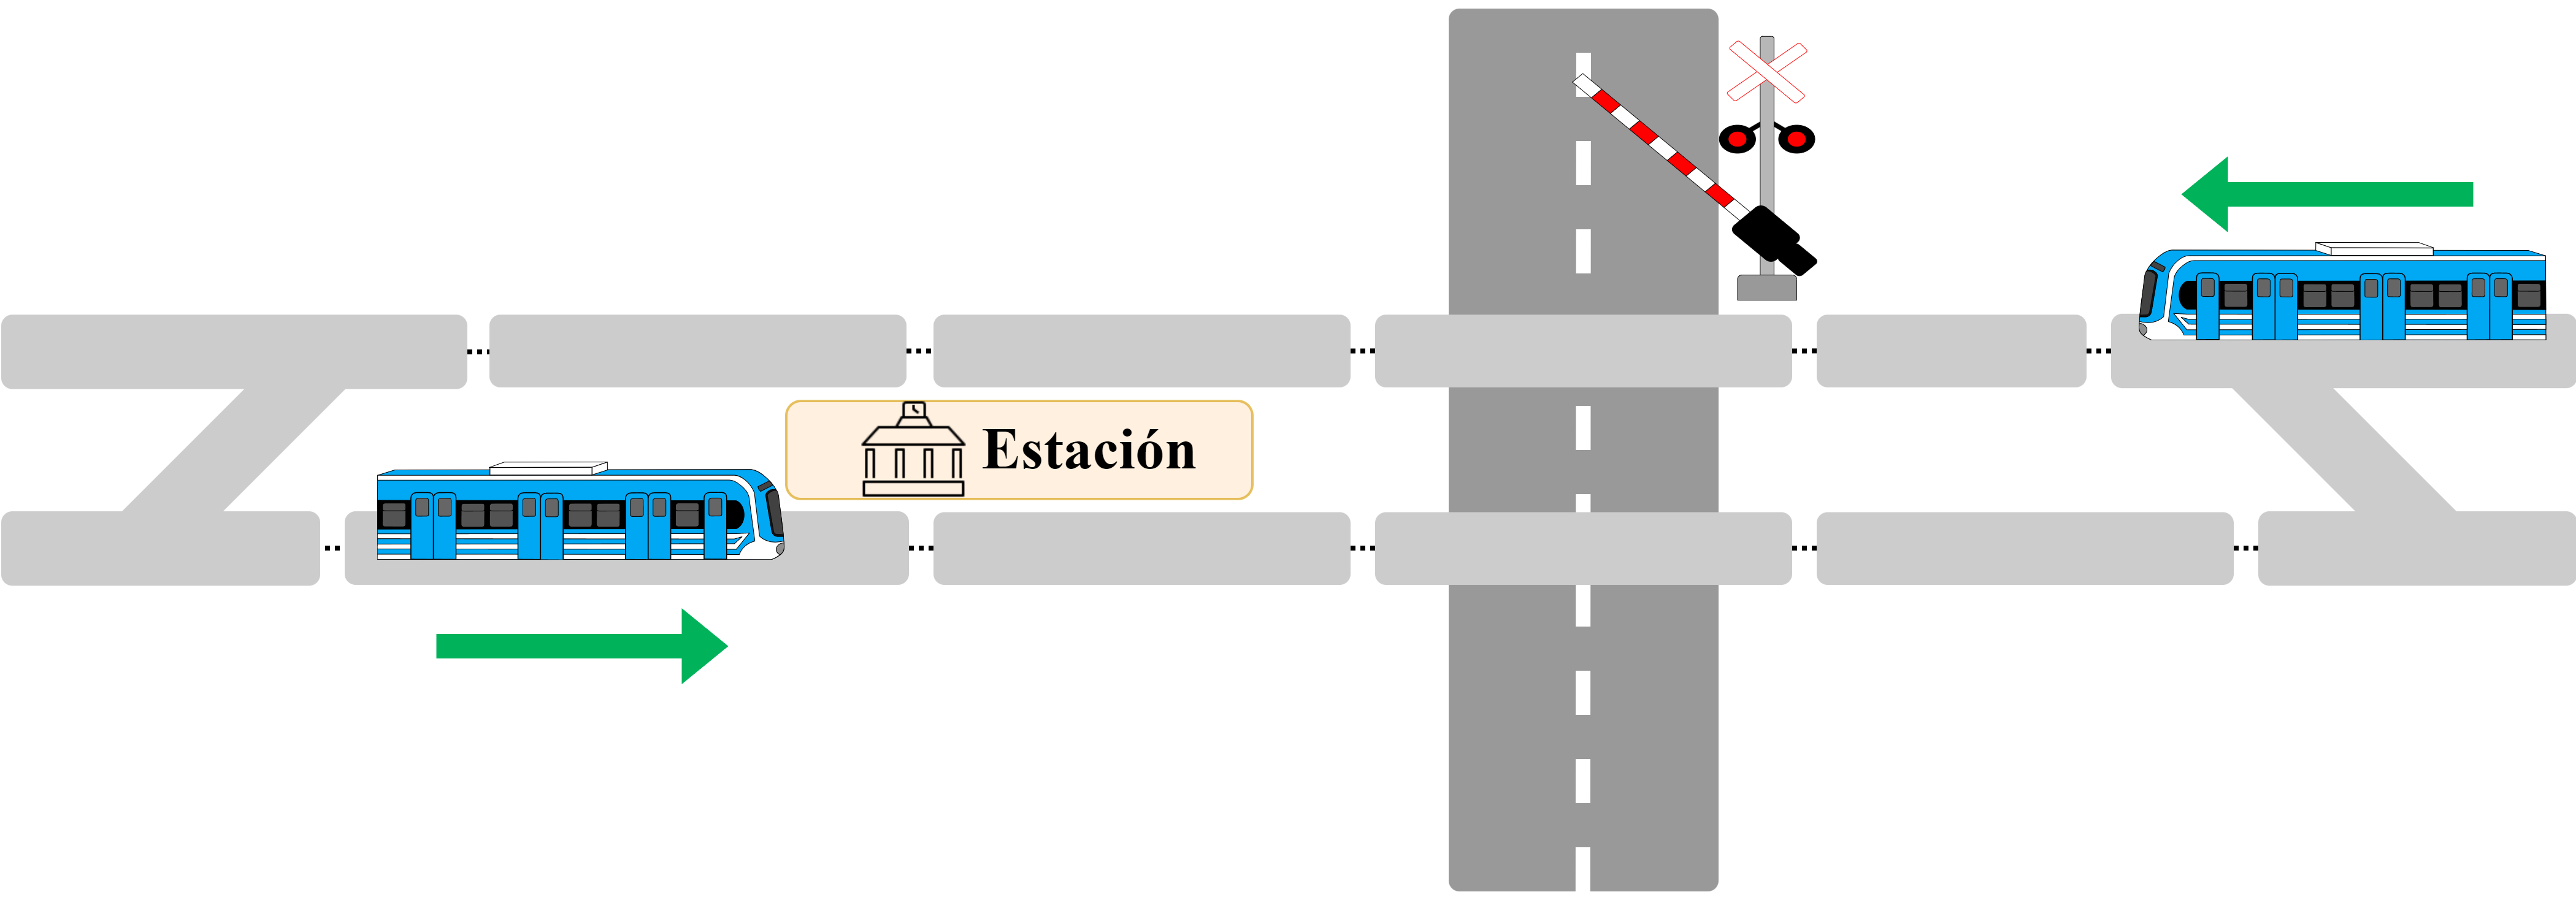
\includegraphics[width=1\textwidth]{Figuras/bajaDensidad}
        \centering\caption{Topología de estación de baja densidad.}
        \label{fig:simple_1}
    \end{figure}

El cruce entre el trazado ferroviario y el trazado vehicular se denomina paso a nivel. El sistema de enclavamientos deberá garantizar que el paso a nivel se encuentre despejado de vehículos y peatones antes de permitir la circulación de trenes sobre este. Esto se logra mediante el uso de una barrera ferroviaria, que baja el brazo de barrera cuando se detectan formaciones ferroviarias en las proximidades del paso a nivel.

Las topologías de estación de baja densidad suelen contar con dos vías unidireccionales en sentido ascendente y descendente. 
Las vías ascendentes son aquellas por las que las formaciones circulan en la dirección del kilometraje creciente. Mientras que las vías descendentes son aquellas por las que circulan en la dirección del kilometraje decreciente \cite{RITO}. El kilómetro cero es la estación principal de la línea ferroviaria, como por ejemplo: Plaza Constitución (Línea Roca), Once de Septiembre (Línea Sarmiento) o Retiro (Línea Mitre y Linea San Martín). Para invertir su sentido de circulación las formaciones pueden cambiar de vía
ascendente a descendente, o viceversa, utilizando un cambio ferroviario